\section{Existing solutions}
\label{sec:altsolution}
Based on the product requirements the team worked out, we did some research on existing solutions in the same market. This resulted in a list of the most relevant solutions, possibly competing with the team's own application.
 
This list contains a brief overview of the functionalities and drawbacks of the existing solutions, summarized in table~\ref{tab:existingSolutions}. The team will use this study in alternative solutions as an inspiration for functionality and features to implement in the project application.


\begin{table}[H]
\centering
\rowcolors{1}{darkgray}{lightgray}
\begin{tabular}{|l|l|p{2.6cm}|p{2.3cm}|p{2.2cm}|}
\hline
\textbf{Product} & \textbf{Device control} & \textbf{Social media} & \textbf{Measure production} & \textbf{Measure individual devices} \\
Smartly & Limited & No  & No & No\\
OpenEnergyMonitor & Yes & No  & Limited & No \\
Minisolo & Yes & No  & No & Limited\\
TheOwl & Yes & No & No & Yes\\
Efergy & Yes & Yes &  No & Yes\\\hline
\end{tabular}
\caption{Comparison of existing solutions}
\label{tab:existingSolutions}
\end{table}


\subsection{NTE miniSolo energydisplay}

The NTE miniSolo energydisplay~\cite{nte} measures the total power usage real time and allows the user to power off devices to see the effect the device has on the total power consumption. It offers some interesting features like detailed power consumption and a relation to how much money the power usage amounts to, which the team also want to have in the application. However, the miniSolo energydisplay has some drawbacks: It is linked to a proprietary device and has no Android application. These drawbacks made the solution incompatible with the team's application.


\subsection{Theowl}

Theowl~\cite{theowl} mainly focuses on temperature control. 
As that was not the only property the team would like to focus on, the solution lacked many of the features the team wanted to have in the application. Other drawbacks is that the product does not have any official support in Norway and also is beyond a reasonable price range. 

However, Theowl has an architecture with remote sensors that sends precise data and allow the user to control certain devices, which the team would like to consider for the application.


\subsection{Smartly}

Smartly~\cite{smartly} allows the user to monitor and control things like temperature and lighting in the house, as shown in figure~\ref{fig:smartlya}. It also has an overview over total power consumption, as shown in figure~\ref{fig:smartlyb}.

Even though Smartly has some of the features the team would like to have in the application, such as being able to turn on and turn off devices, has a good design and has a display of money saved caused by use of the application, it does not offer the ability to measure the power usage in each device, which was a high-priority feature in the team's application.


\begin{figure}[H]
\addcontentsline{lof}{figure}{2.1\hspace{4mm}Smartly screenshots}
\label{fig:smartly}
  \centering
  \subbottom[\label{fig:smartlya}Screenshot of Smartly's possibility to remotely control devices.]{%
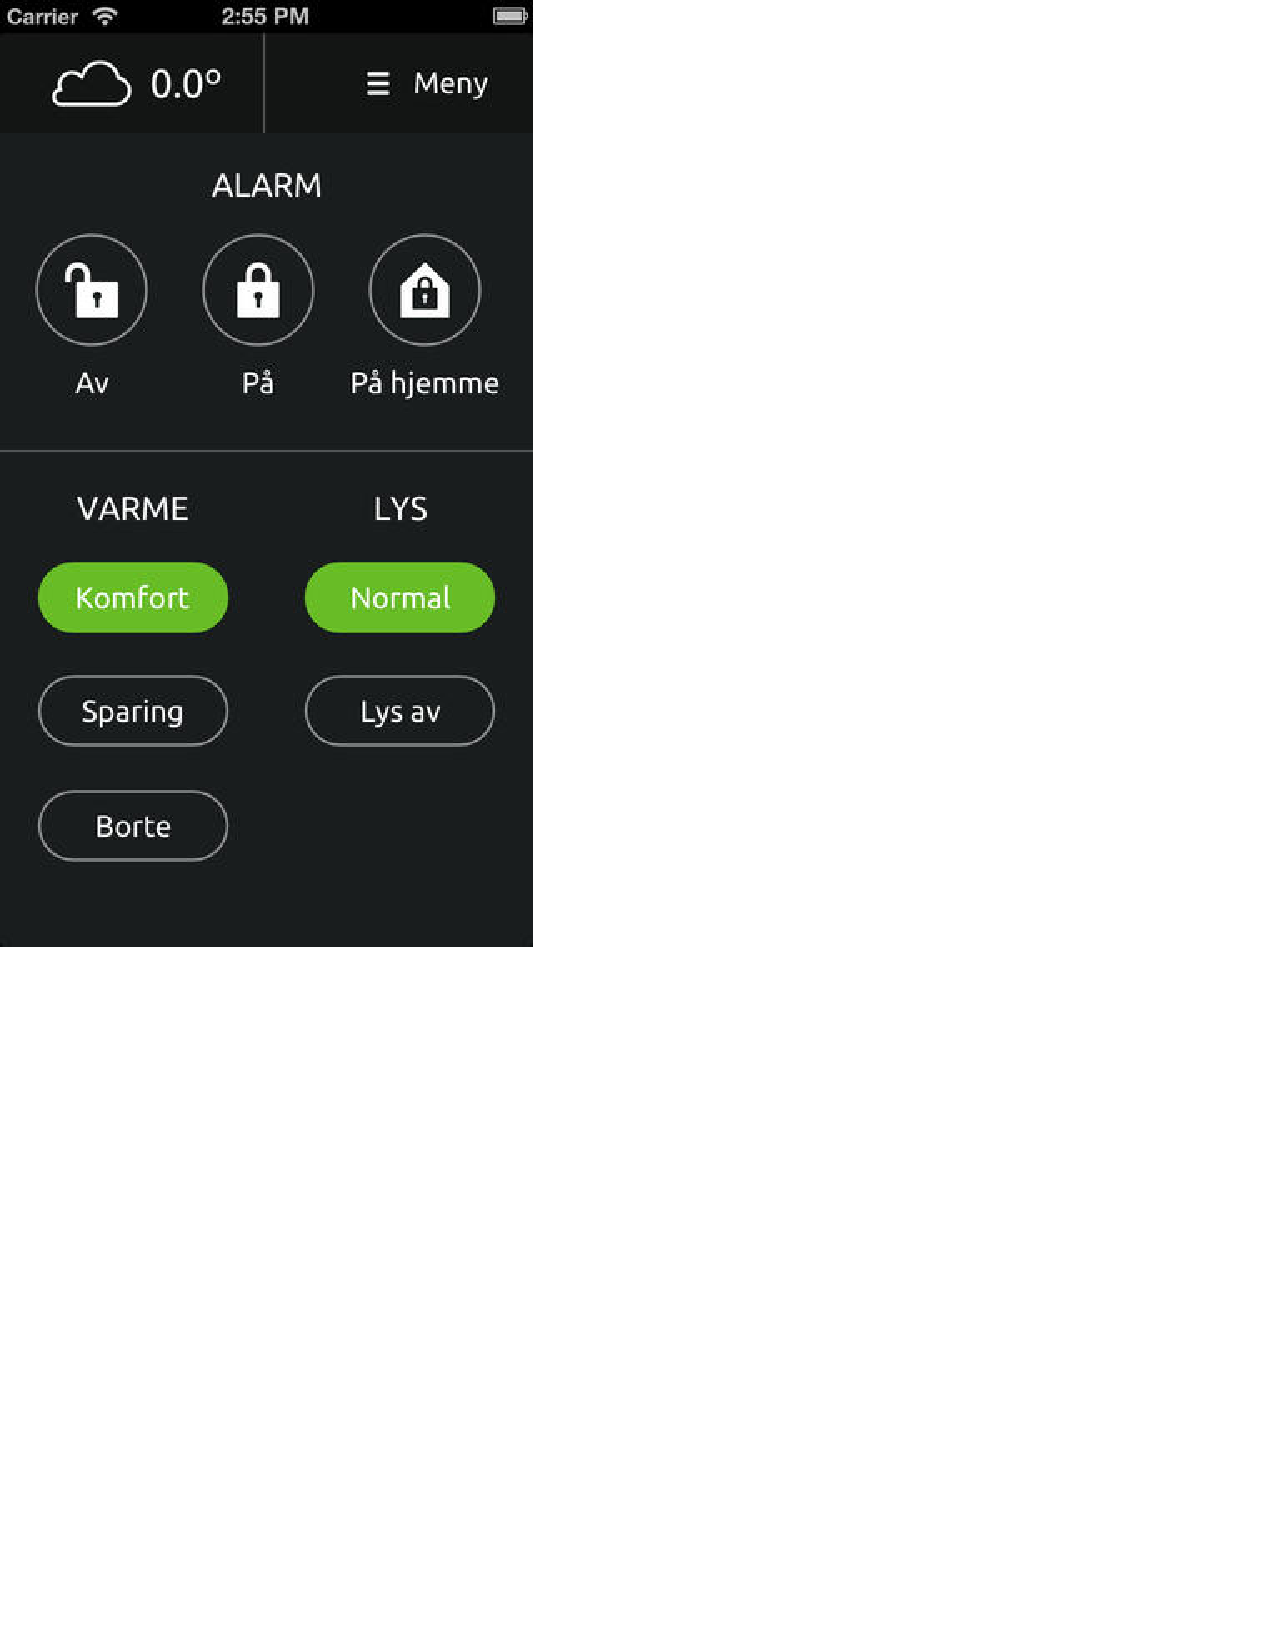
\includegraphics[width=0.45\textwidth, trim=0cm 12cm 13cm 0cm, clip]{ch/prestudy/fig/smartlyLock.pdf}}
\quad
  \subbottom[\label{fig:smartlyb} Screenshot of Smartly's consumption overview.]{%
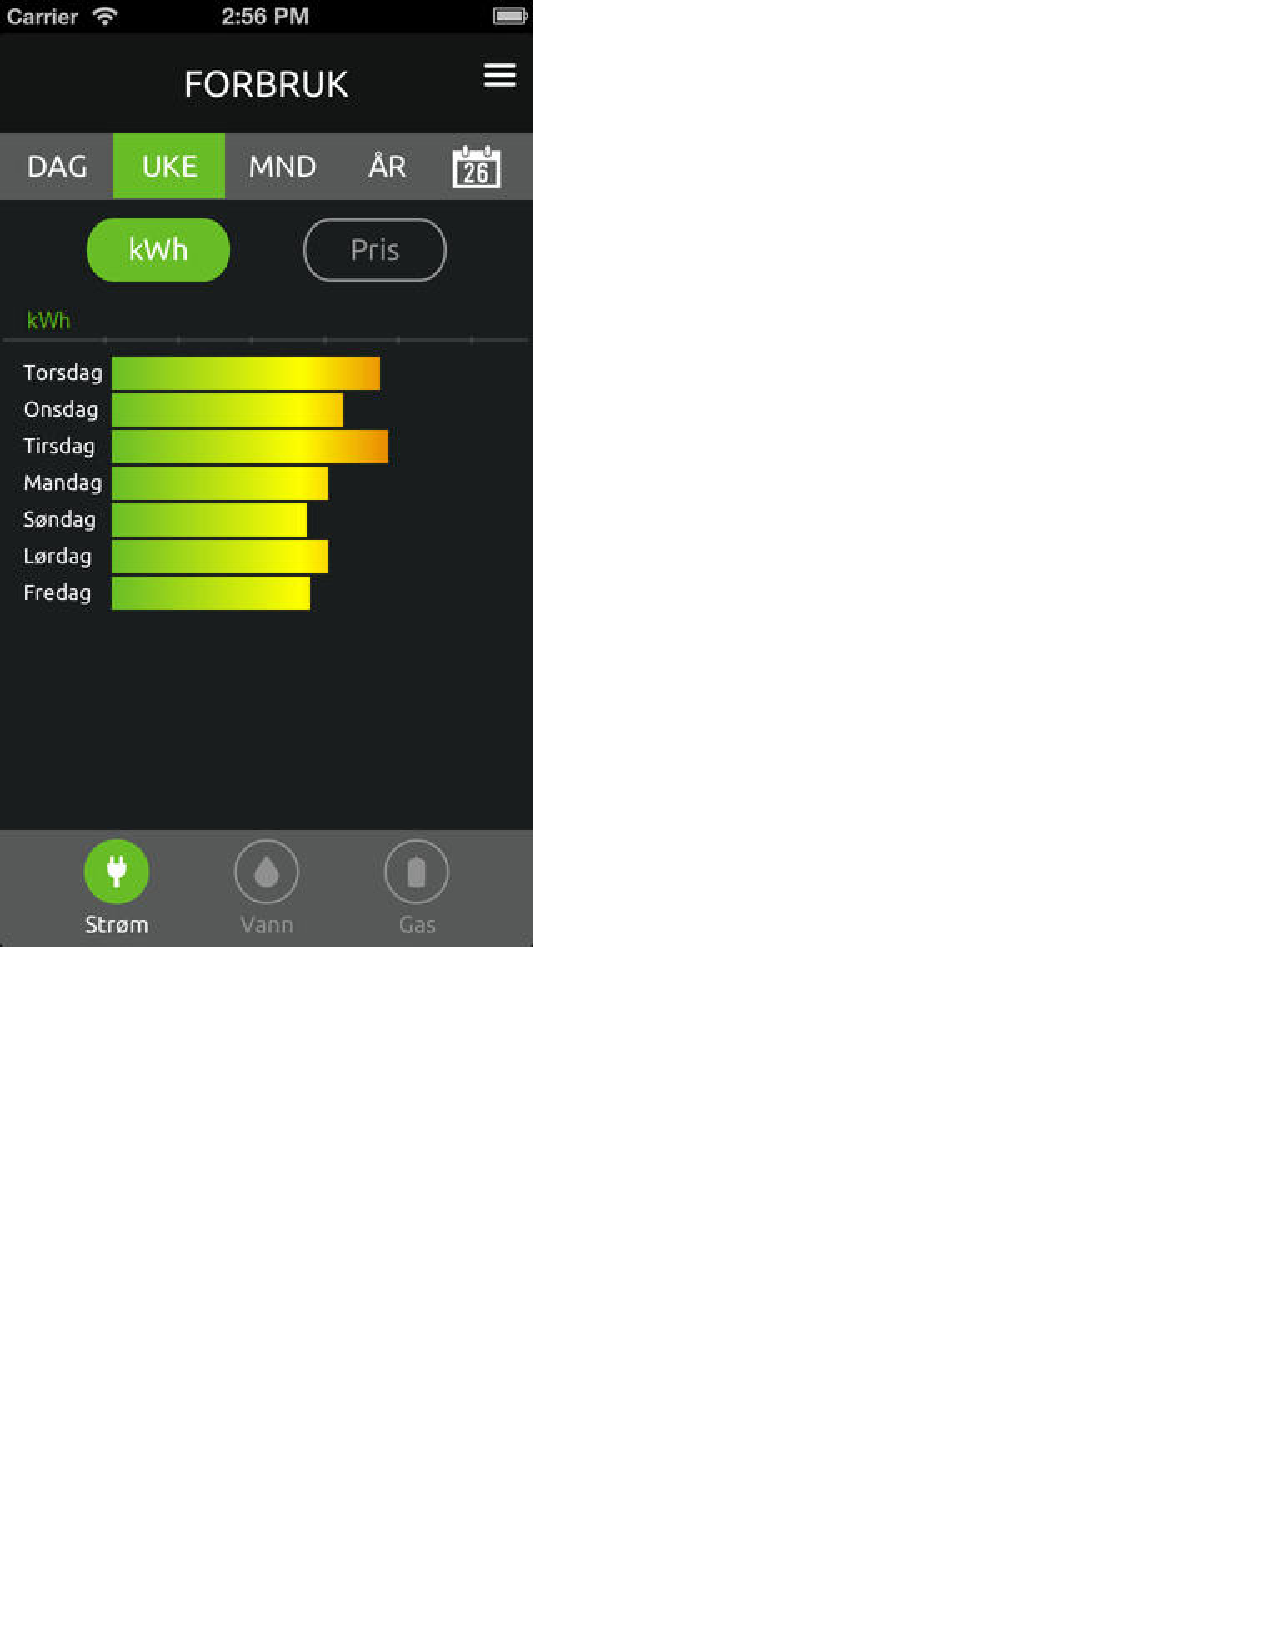
\includegraphics[width=0.45\textwidth, trim=0cm 12cm 13cm 0cm, clip]{ch/prestudy/fig/smartlyConsume.pdf}}
\end{figure}


\subsection{OpenEnergyMonitor}

OpenEnergyMonitor~\cite{openenergymonitor} is an open source project that allows data collection from power outages. Some of the architecture for collecting data can be an interesting option to consider if improved. The architecture, shown in figure~\ref{fig:oem}, is somewhat similar to what the team itself imagined to use in the application. 

However, OpenEnergyMonitor offers no automatic collection of data - the user would have to manually go around his house to collect the data. It is also somewhat hard to set up, which would make the solution not very user friendly for the average consumer. This solution also has an application for processing, logging and visualizing energy usage. These are features the team wanted to have in the application.

\setcounter{figure}{1}
\begin{figure}[H]
\centering
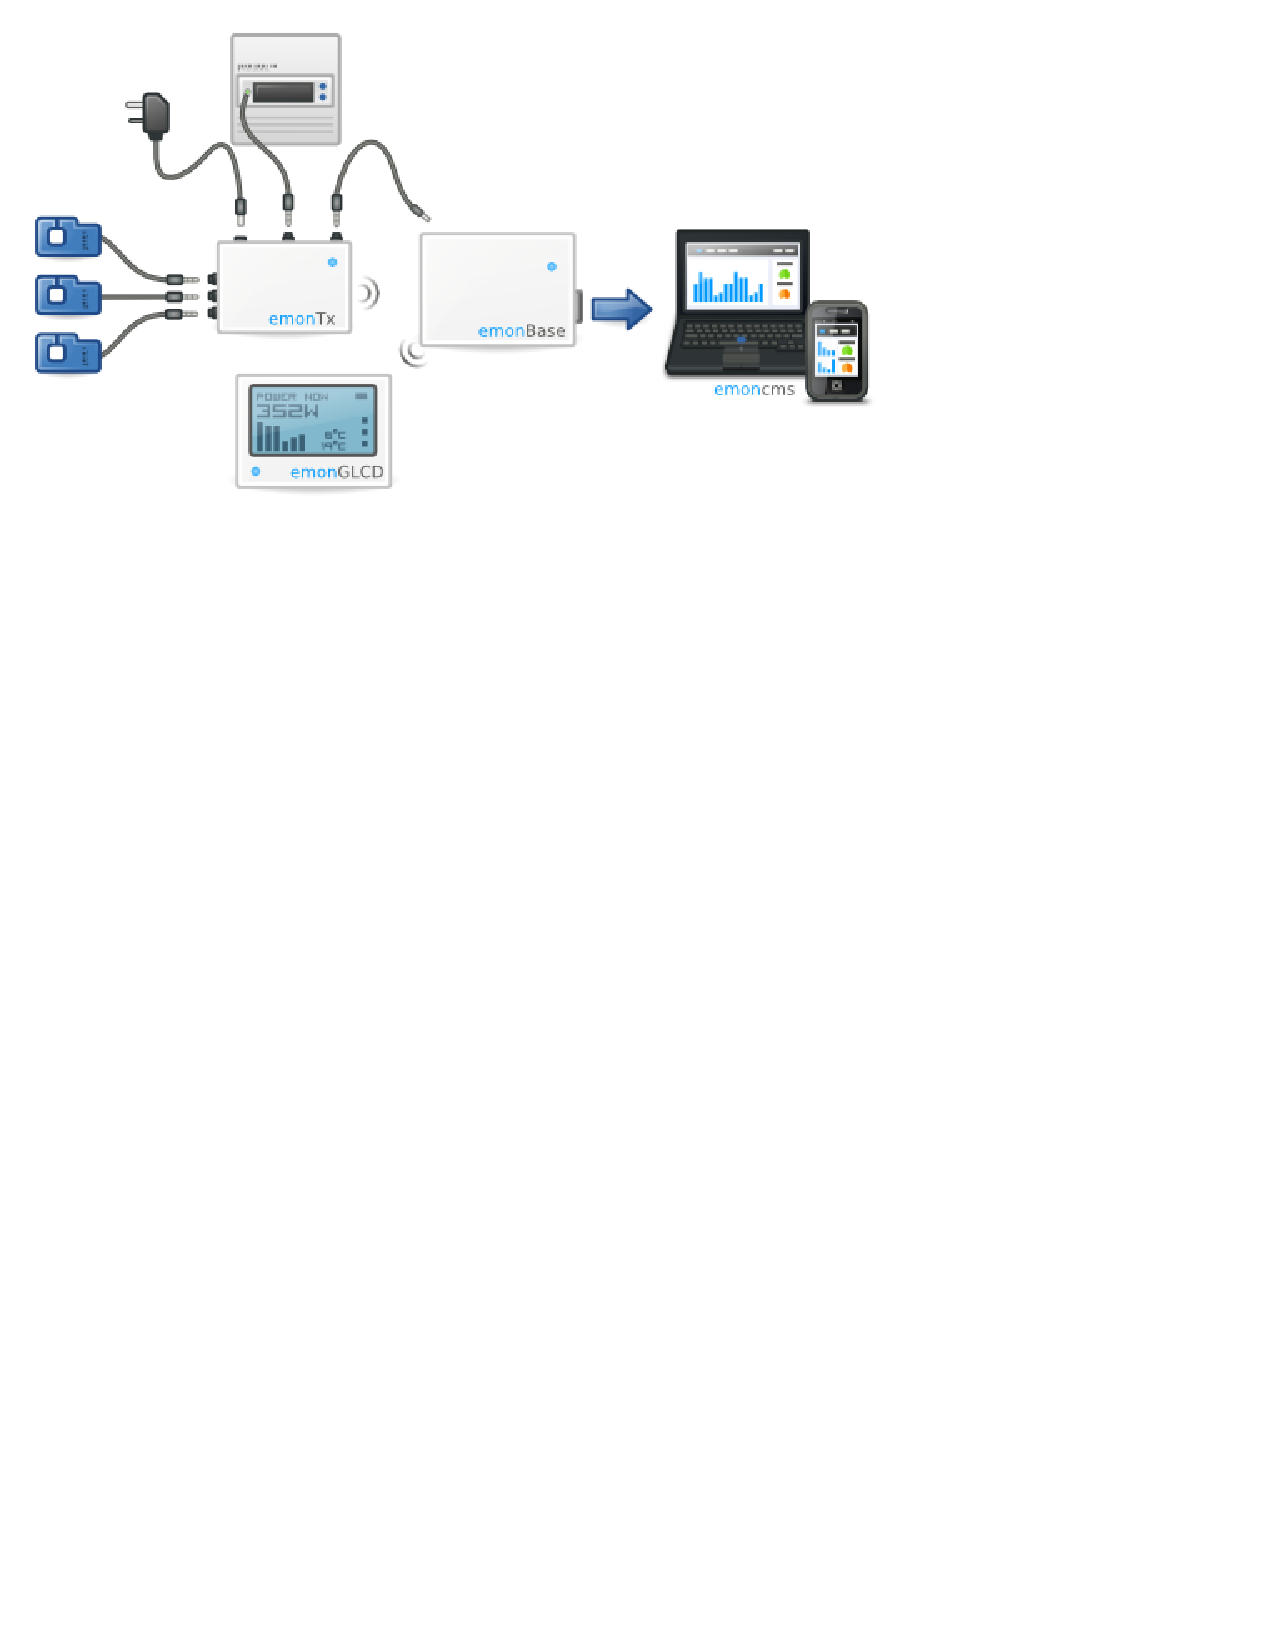
\includegraphics[width=\textwidth, trim=0.5cm 19cm 6.5cm 0cm, clip]{ch/prestudy/fig/OEM_system.pdf}
\caption{OpenEnergyMonitor's system architecture}
\label{fig:oem}
\end{figure}




\newpage
\subsection{Efergy}

Efergy~\cite{efergy} was considered to be the closest solution to what the team wanted to develop. As shown in figure~\ref{fig:efergyGUI}, it has nice visual representation of data, and it offers social integration. The architecture is interesting, as it supports measuring the power usage of single devices over wireless radio, communicating with a local receiver. The receiver is connected to a server through the user's Internet. Unfortunately, it lacks the ability to monitor and control private power production. It is also beyond a reasonable price range.

\begin{figure}[H]
\centering
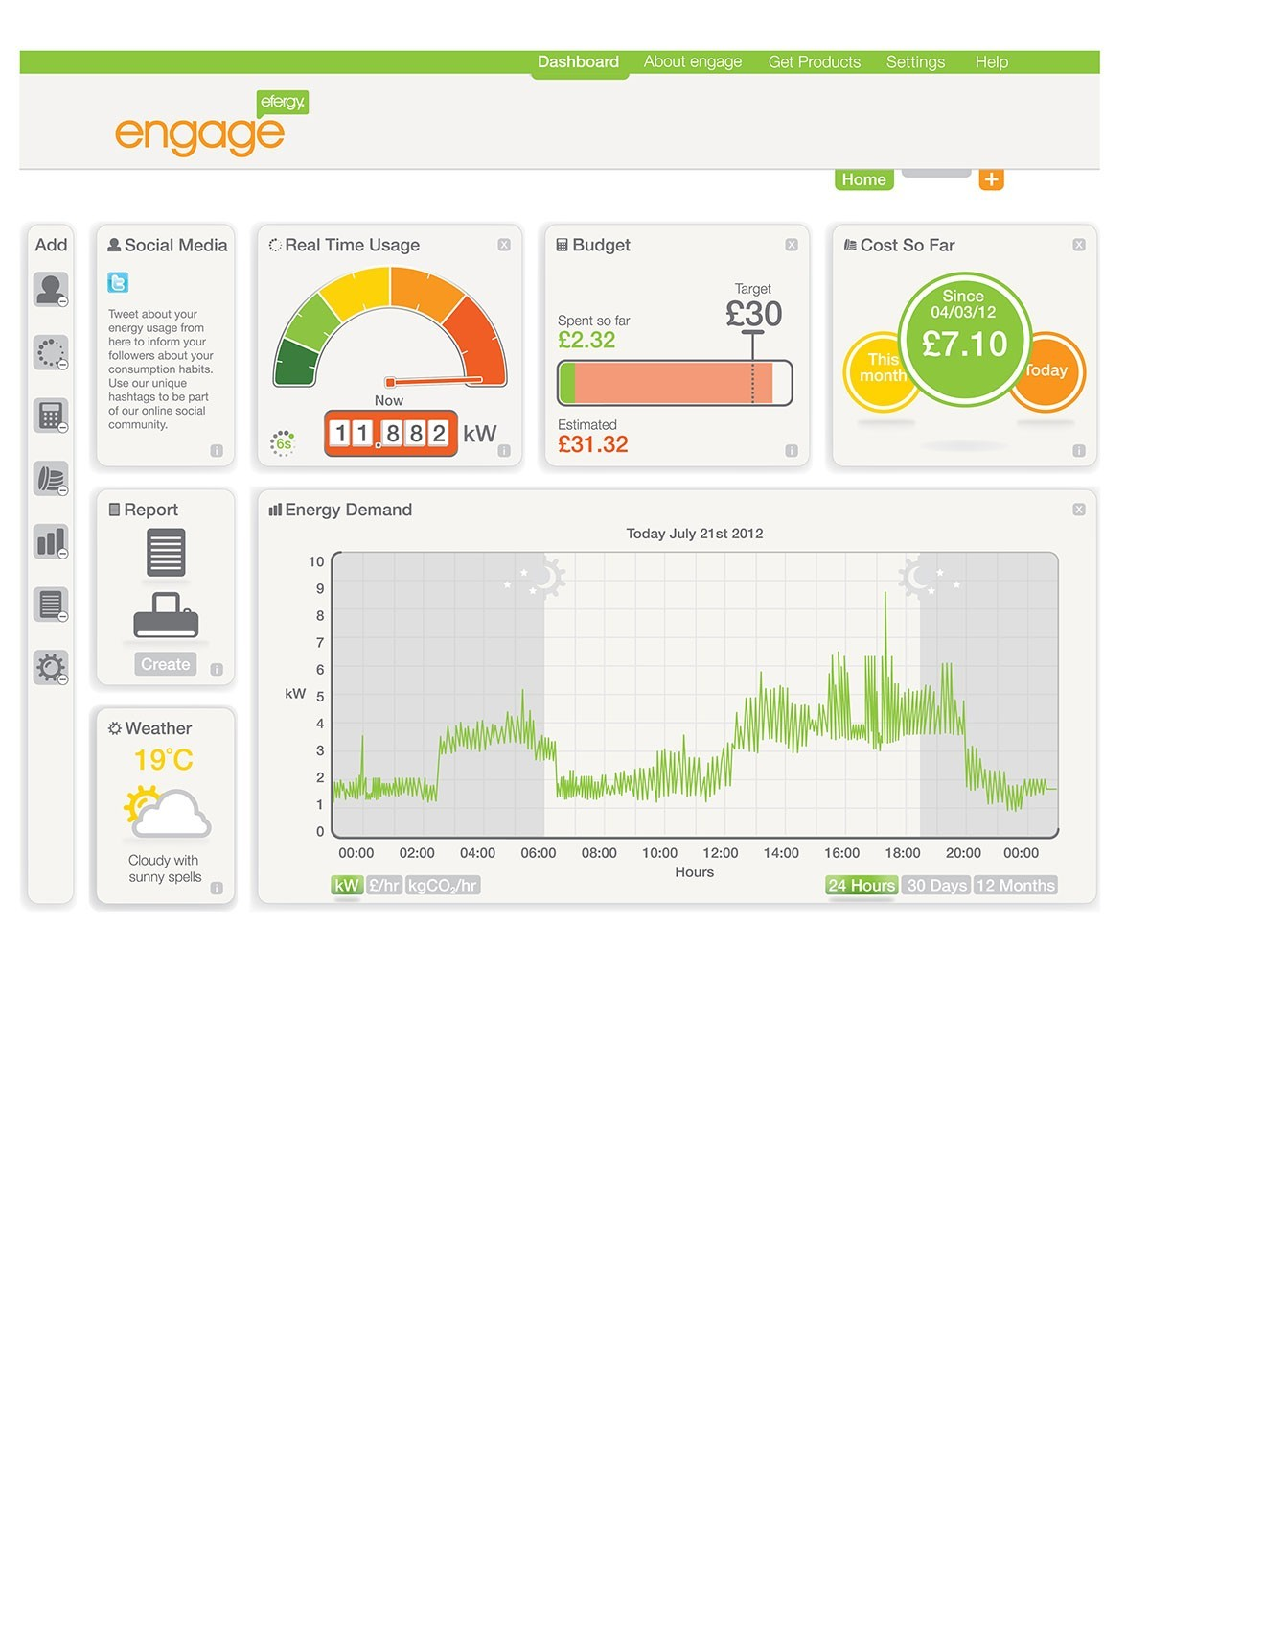
\includegraphics[width=10cm, trim=0.5cm 12cm 3cm 0.7cm, clip]{ch/prestudy/fig/efergy.pdf}
\caption{Screenshot of the Efergy Engage GUI}
\label{fig:efergyGUI}
\end{figure}


